\documentclass{article}
\usepackage{ctex}
\usepackage[a4paper, total={6in, 8in}]{geometry}
\setlength{\parindent}{0pt}
\usepackage{amsmath,amssymb,amsfonts,color}
\usepackage{bm}
\usepackage{graphicx}
\usepackage{float} 
\usepackage{caption} 
\usepackage{subfigure}
\usepackage{algorithm}
\usepackage[document]{ragged2e}
\usepackage{xcolor}
\usepackage{setspace}
\usepackage{listings}
\setstretch{1.8}
\setlength{\parindent}{2em}
\begin{document}
{\centering\section*{优化方法第三章作业}}
\textcolor{blue}{1. 假设函数$f$ 是满足 $ mI \leq \nabla^2 f(x) \leq MI$的强凸函数。令$d$为$x$处的下降方向。证明对于 
$0<t \leq -\frac{\nabla^2 f(x)^Td}{M\Vert d \Vert_2^2}$回溯终止条件能够满足}\\
1. 证明:
$f$在$x$处二阶展开有 $f(x+td) \approx f(x) + t \nabla f(x)^T d + \frac{t^2}{2}d^t\nabla^2 f(x)d$\\
由于f满足$ mI \leq \nabla^2 f(x) \leq MI$,故\\
$f(x) + t \nabla f(x)^T d + \frac{t^2}{2}d^t\nabla^2 f(x)d \leq f(x) + t \nabla f(x)^T d + \frac{t^2}{2}M\Vert d \Vert_2^2$\\
故当$f(x) + t \nabla f(x)^T d + \frac{t^2}{2}M\Vert d \Vert_2^2 \leq f(x) + \alpha t \nabla f(x)^T d$时,回溯条件满足\\
因为$t > 0$,化简得$(1-\alpha)\nabla f(x)^T d  +  \frac{t}{2}M\Vert d \Vert_2^2ß \leq 0$\\
因为$0 < \alpha < \frac{1}{2}$, 所以$ 0 < t \leq -\frac{\nabla^2 f(x)^Td}{M\Vert d \Vert_2^2}$\\


\textcolor{blue}{2. 假设存在$m,M$满足$mI \leq \nabla^2 f(x) \leq MI (\forall x \in S)$;\\
存在常数$\gamma,\tilde{\gamma} \in (0,1]$,使得 $\Vert x \Vert \geq \gamma \Vert x \Vert_2, \Vert x \Vert_* \geq \tilde{\gamma}\Vert x \Vert_2$ \\
证明:\\
1). 精确直线搜索时,非规范化最速下降方法的收敛性.\\ 
2). 回溯直线搜索时,非规范化最速下降方法的收敛性.}\\
证明:
1)$f$在$x$处二阶展开有 $f(x^k+td^k_{sd}) \approx f(x^k) + t \nabla f(x^k)^T d^k_{sd} + \frac{t^2}{2}d^k_{sd}\nabla^2 f(x^k)d^k_{sd}$\\
由于f满足$ mI \leq \nabla^2 f(x) \leq MI$\\
故$f(x^k+td^k_{sd}) \leq f(x^k) + t \nabla f(x^k)^T d^k_{sd} + \frac{t^2}{2}M\Vert d^k_{sd} \Vert_2^2$\\
等式右侧对$t$取最小值得:$f(x_{k+1}) \leq f(x^k) - \frac{1}{2M}\Vert \nabla f(x^k)\Vert ^2_2$.\\
故$f(x^k)  \geq  f(x^{k+1}) + \frac{1}{2M}\Vert \nabla f(x^k)\Vert ^2_2$\\
先证明若$mI \leq \nabla^2 f(x)$,有$f(x) - p^* \leq \frac{1}{2m}\Vert \nabla f(x)\Vert^2_2$\\
$f(y) \approx f(x) + \nabla f(x)^T (y-x) + \frac{1}{2}(y-x)^T \nabla^2 f(x) (y-x) \geq f(x) + \nabla f(x)^T (y-x) + \frac{m}{2} \Vert (y-x)\Vert_2^2$\\
右侧为关于y的凸函数,令右侧对y求导等于0得$\tilde{y} = x - \frac{1}{m}\nabla f(x)$\\
故$f(y) \geq f(x) + \nabla f(x)^T (y-x) + \frac{m}{2} \Vert (y-x)\Vert_2^2 \geq f(x) + \nabla f(x)^T (\tilde{y}-x) + \frac{m}{2} \Vert (\tilde{y}-x)\Vert_2^2 = f(x) - \frac{1}{2m}\Vert \nabla f(x)\Vert^2_2$\\
所以$\forall y \in S, f(x) - f(y) \leq \frac{1}{2m} \Vert \nabla f(x)\Vert^2_2$\\
故$f(x) - p^* \leq \frac{1}{2m} \Vert \nabla f(x)\Vert^2_2$\\
变换得:$\Vert \nabla f(x)\Vert^2_2 \geq 2m(f(x) - p*)$\\
因为$f(x^k)  \geq  f(x^{k+1}) + \frac{1}{2M}\Vert \nabla f(x^k)\Vert ^2_2$,左右两侧同时减去$p_*$\\
得:$f(x^k) -p^* \geq  f(x^{k+1}) - p^* + \frac{1}{2M}\Vert \nabla f(x^k)\Vert ^2_2$\\
将$\Vert \nabla f(x)\Vert^2_2 \geq 2m(f(x) - p*)$代入\\
得:$f(x^k) -p^* \geq  f(x^{k+1}) - p^* + \frac{m}{M}(f(x^k) - p^*)$\\
故$f(x^{k+1}) - p^* \leq  (1 - \frac{m}{M})(f(x^k) - p^*)$\\
迭代得$f(x^{k+1}) - p^* \leq (1 - \frac{m}{M})^{k+1}(f(x^0) - p^*)$\\
用$k$替换$k+1$得:$f(x^k) - p^* \leq (1 - \frac{m}{M})^k(f(x^0) - p^*)$\\
算法收敛时:$f(x^k) -p^* \leq \epsilon$得 \textcolor{red}{$K \geq \frac{log((f(x^0) - p^*)/\epsilon)}{\vert log(1-\frac{m}{M}) \vert }$}\\
$\frac{log((f(x^0) - p^*)/\epsilon)}{\vert log(1-\frac{m}{M}) \vert }$ 即为精确直线搜索,非规范化最速下降方法的收敛次数的上界。\\



2)$f$在$x$处二阶展开有 $f(x^k+td^k_{sd}) \approx f(x^k) + t \nabla f(x^k)^T d^k_{sd} + \frac{t^2}{2}d^k_{sd}\nabla^2 f(x^k)d^k_{sd}$\\
由于f满足$ mI \leq \nabla^2 f(x) \leq MI$\\
故$f(x^k+td^k_{sd}) \leq f(x^k) + t \nabla f(x^k)^T d^k_{sd} + \frac{t^2}{2}M\Vert d^k_{sd} \Vert_2^2$\\
因为$\gamma \in (0,1]$\\
故$f(x^k) + t \nabla f(x^k)^T d^k_{sd} + \frac{t^2}{2}M\Vert d^k_{sd} \Vert_2^2 
\leq f(x^k) + t \nabla f(x^k)^T d^k_{sd} + \frac{t^2}{2 \gamma ^2}M\Vert d^k_{sd} \Vert_2^2$\\
因为 $\Vert \nabla f(x^k)^T d^k_{sd} \Vert = - \Vert \nabla f(x^k) \Vert^2_* , \Vert d^k_{sd} \Vert =
\Vert \Vert \nabla f(x^k) \Vert_* \times d^k_{nsd} \Vert = \Vert \nabla f(x^k) \Vert_* \Vert d^k_{nsd} \Vert = \Vert \nabla f(x^k) \Vert_*$\\
所以 $f(x^k) + t \nabla f(x^k)^T d^k_{sd} + \frac{t^2}{2 \gamma ^2}M\Vert d^k_{sd} \Vert_2^2 = f(x^k) - t \Vert \nabla f(x^k) \Vert_*^2 + \frac{Mt^2}{2 \gamma ^2} \Vert \nabla f(x^k) \Vert_* ^2$\\
对两边同时对$t$取最小值得:$t = \frac{\gamma ^2}{M}$, $\alpha < \frac{1}{2}$ \\
$(x^k+t_{min}d^k_{sd}) \leq f(x^k) - \frac{1}{2}t_{min}\Vert \nabla f(x^k) \Vert_* ^2 \leq f(x^k) + \alpha t_{min} \nabla f(x^k)^T d^k_{sd}$\\
当回溯直线搜索停止时$ t \geq min\{ 1, \frac{\beta \gamma ^2 }{M}\}$,有:\\
$f(x^{k+1}) = f(x^k+td^k_{sd}) \leq f(x^k) - \alpha min\{ 1, \frac{\beta \gamma ^2}{M}\} \Vert \nabla f(x^k) \Vert_* ^2 \leq f(x^k) - \alpha \tilde{\gamma}^2 min\{ 1, \frac{\beta \gamma ^2}{M}\} \Vert \nabla f(x^k) \Vert_2 ^2$
两边同时减最优值$p^*$,有:\\
$f(x^{k+1}) - p^* \leq f(x^k) - p^* - \alpha \tilde{\gamma}^2 min\{ 1, \frac{\beta \gamma ^2}{M}\} \Vert \nabla f(x^k) \Vert_2 ^2$\\
因为$mI \leq \nabla^2 f(x)$,故$f(x^k) - p^* \leq \frac{1}{2m}\Vert \nabla f(x^k) \Vert_2 ^2$\\
故$f(x^{k+1}) - p^* \leq (1 - 2m \alpha \tilde{\gamma} ^2 min\{1,\frac{\beta \gamma ^2 }{M}\})(f(x^k) - p^*)$\\
令$c = 1 - 2m \alpha \tilde{\gamma} ^2 min\{1,\frac{\beta \gamma ^2 }{M}\}$\\
故$f(x^{k+1}) -p^* \leq c f(x^k) - p^*$\\
迭代得:$f(x^{k+1})-p^* \leq c^{k+1} (f(x^0) - p^*)$\\
用$k$替换$k+1$得:$f(x^k) -p^* \leq c^k (f(x^0) - p^*)$\\
算法收敛时:$f(x^k) -p^* \leq \epsilon$得 \textcolor{red}{$K \geq \frac{log((f(x^0) - p^*)/\epsilon)}{log(1/c)}$}\\
$\frac{log((f(x^0) - p^*)/\epsilon)}{log(1/c)}$ 即为回溯直线搜索,非规范化最速下降方法的收敛次数的上界。\\

\newpage
\textcolor{blue}{3. 假设存在$m,M$满足$mI \leq \nabla^2 f(x) \leq MI (\forall x \in S)$;\\
存在$L$满足$\Vert \nabla^2 f(y)  - \nabla^2 f(x)\Vert_2  \leq L \Vert y-x \Vert_2 (\forall x,y \in S)$\\
证明:回溯直线搜索时,牛顿方法的收敛性 }\\
证明:\\
阻尼牛顿阶段:要证明$0 < \eta \leq \frac{m^2}{L} , \Vert \nabla f(x^k) \Vert_2 \geq \eta $时 $f(x^{k+1}) - f(x^k) \leq -\gamma (\gamma > 0)$\\
证明:$f$在$x$处二阶展开有 $f(x^k+td^k_{nt}) \approx f(x^k) + t \nabla f(x^k)^T d^k_{nt} + \frac{t^2}{2}d^t\nabla^2 f(x^k)d$\\
由于$f$满足$\nabla^2 f(x) \leq MI$\\
故$f(x^k+td^k_{nt}) \leq f(x^k) + t \nabla f(x^k)^T d^k_{nt} + \frac{t^2}{2}M\Vert d^k_{nt} \Vert_2^2$\\
根据牛顿下降方向的定义 $ \nabla f(x^k)^T d^k_{nt} = -\lambda(x^k)^2, \lambda(x^k)^2 = (d^k_{nt})^T \nabla^2 f(x^k) d^k_{nt} \geq m \Vert d^k_{nt}\Vert_2^2$\\
故$f(x^k) + t \nabla f(x^k)^T d^k_{nt} + \frac{t^2}{2}M\Vert d^k_{nt} \Vert_2^2 \leq f(x^k) - t \lambda(x^k)^2 + \frac{M}{2m}t^2 \lambda(x^k)^2 $\\
对两边同时对$t$ 取最小值得:$ f(x^k + t_{min}d^k_{nt}) \leq f(x^k) - \frac{m}{2M}  \lambda(x^k)^2 \leq f(x^k) - \alpha \frac{m}{M}  \lambda(x^k)^2 $ \\$(t_{min} = \frac{m}{M})$\\
回溯直线搜索停止$t \geq \beta t_{min} = \beta \frac{m}{M}$ 有:\\
$f(x^{k+1}) - f(x^k) = f(x^k+td^k_{nt}) - f(x^k) \leq -\alpha t \lambda(x^k)^2 \leq -\alpha \beta \frac{m}{M} \lambda(x^k)^2 $\\
因为$ \lambda(x^k)^2 =  \nabla f(x^k)^T  \nabla^2 f(x^k)^{-1}  \nabla f(x^k) \geq \frac{1}{M} \Vert  \nabla f(x^k) \Vert_2^2$\\
故$f(x^{k+1}) - f(x^k) \leq -\alpha \beta \frac{m}{M} \lambda(x^k)^2 \leq -\alpha \beta \frac{m}{M^2} \Vert  \nabla f(x^k) \Vert_2^2 \leq -\alpha \beta \eta ^2\frac{m}{M^2}$\\
取$\gamma = \alpha \beta \eta ^2\frac{m}{M^2}$得证\\
二次收敛阶段:要证明$\Vert  \nabla f(x^k) \Vert_2 < \eta$时,$t^k = 1, \frac{L}{2m^2}\Vert  \nabla f(x^{k+1}) \Vert_2 \leq (\frac{L}{2m^2}\Vert  \nabla f(x^k) \Vert_2)^2$\\
证明:函数$f$的$Hessian$矩阵以$L$为常数的$Lipcshitz$连续,即存在$L>0$,使得$\Vert  \nabla^2(y) - \nabla^2(x)\Vert_2 \leq L\Vert y-x\Vert_2$\\
有$\Vert \nabla^2(x^k + t d^k_{nt}) - \nabla^2(x^k)\Vert_2 \leq tL \Vert d^k_{nt} \Vert_2$
两侧同时左乘$( d^k_{nt})^T$,右乘$ d^k_{nt}$得\\
$( d^k_{nt})^T \Vert \nabla^2(x^k + t d^k_{nt}) - \nabla^2(x^k)\Vert_2 d^k_{nt} \leq tL \Vert d^k_{nt} \Vert_2^3 $\\
令$\tilde{f}(t) = f(x^k + td^k_{nt})$有$\tilde{f}''(t) = ( d^k_{nt})^T\nabla^2(x^k + t d^k_{nt}) d^k_{nt}$\\
$\tilde{f}''(0) = \lambda(x^k)^2 \geq m\Vert d^k_{nt} \Vert_2^2$\\
$\tilde{f}'(0) = -\lambda(x^k)^2$\\
故$\vert \tilde{f}''(t) - \tilde{f}''(0)  \vert \leq tL \Vert d^k_{nt} \Vert_2^3$\\
$\tilde{f}''(t) \leq \tilde{f}''(0) + tL \Vert d^k_{nt} \Vert_2^3 \leq \lambda(x^k)^2 + \frac{tL}{m^{\frac{3}{2}}}\lambda(x^k)^3$\\
将$\tilde{f}'(t)$一阶泰勒展开有:$\tilde{f}'(t) = \tilde{f}'(0) + t \tilde{f}''(0) \leq \tilde{f}'(0) + t\lambda(x^k)^2 + \frac{t^2L}{m^{\frac{3}{2}}}\lambda(x^k)^3 = -\lambda(x^k)^2 + t\lambda(x^k)^2 + \frac{t^2L}{m^{\frac{3}{2}}}\lambda(x^k)^3 $\\
故$\tilde{f}(t) \leq \tilde{f}(0) - t\lambda(x^k)^2 + \frac{1}{2}t^2 \lambda(x^k)^2+ \frac{t^3L}{6m^{\frac{3}{2}}}\lambda(x^k)^3 $\\
令$t = 1$,同时将$\tilde{f}(t) =f(x^k + td^k_{nt}) $还原得:\\
$f(x^k + td^k_{nt}) \leq f(x^k) - \lambda(x^k)^2 (\frac{1}{2} - \frac{L \lambda(x^k)}{6m^{\frac{3}{2}}})\leq f(x^k) - \alpha \lambda(x^k)^2 = f(x^k) + \alpha \nabla f(x^k)^T d^k_{nt}$\\
故满足回溯直线搜索停止条件,$x^{k+1} = x^k + d^k_{nt}$\\
若$\Vert \nabla f(x^k) \Vert_2 \leq \eta \leq 3(1-2\alpha)\frac{m^2}{L}$\\
则$\lambda(x^k) = (\nabla f(x^k)^T \nabla^2f(x^k)^{-1} \nabla f(x^k) )^{1/2} \leq \frac{1}{m^{1/2}} \Vert \nabla f(x^k) \Vert_2 \leq 3(1-2\alpha)\frac{m^2}{L}$\\
下面证明:$\frac{L}{2m^2}\Vert  \nabla f(x^{k+1}) \Vert_2 \leq (\frac{L}{2m^2}\Vert  \nabla f(x^k) \Vert_2)^2$\\
$\nabla f(x^{k+1}) = \nabla f(x^k + d^k_{nt}) = \nabla f(x^k + d^k_{nt}) - \nabla f(x^k) - \nabla^2 f(x^k)d^k_{nt}$\\
$\Vert \nabla f(x^{k+1}) \Vert_2 = \Vert \int_{0}^{1} (\nabla^2 f(x^k + td^k_{nt}) - \nabla^2 f(x^k))d^k_{nt} dt \Vert_2 \leq \int_{0}^{1} Lt\Vert d^k_{nt}\Vert_2^2 = \frac{L}{2}\Vert d^k_{nt}\Vert_2^2 = \frac{L}{2}\Vert \nabla ^2 f(x^k) ^{-1} \nabla f(x^k)\Vert_2^2 \leq \frac{L}{2m^2}\Vert  \nabla f(x^k) \Vert_2^2$\\
如果存在$\tilde{k}, \Vert  \nabla f(x^{\tilde{k}}) \Vert_2 < \eta$,那么$\forall K \geq \tilde{k},\Vert  \nabla f(x^K) \Vert_2 < \eta$\\
又因为$\frac{L}{2m^2}\Vert  \nabla f(x^{K+1}) \Vert_2 \leq (\frac{L}{2m^2}\Vert  \nabla f(x^K) \Vert_2)^2$\\
所以$\frac{L}{2m^2}\Vert  \nabla f(x^{K}) \Vert_2 \leq (\frac{L}{2m^2}\Vert  \nabla f(x^{\tilde{k}}) \Vert_2)^{2^{K - \tilde{k}}}\leq (\frac{1}{2})^{2^{K-\tilde{k}}}$\\
又因为$\Vert  \nabla f(x^{\tilde{k}}) \Vert < \eta = min\{1,3(1-2\alpha)\}\frac{m^2}{L}$\\
所以$f(x^K) - p^* \leq \frac{1}{2m} Vert  \nabla f(x^K) \Vert_2^2 \leq \frac{2m^3}{L^2}(\frac{1}{2})^{2^{K-\tilde{k} + 1}}$\\
记$\epsilon_0 = \frac{2m^3}{L^2}, K_2 = K-\tilde{k} + 1$,$f(x^K) - p^* \leq \frac{2m^3}{L^2}(\frac{1}{2})^{2^{K-\tilde{k} + 1}} \leq \epsilon$\\
所以$k_2 \geq log_2(log_2(\epsilon_0 / \epsilon))$\\
所以,总迭代次数:$K \geq \frac{f(x^0) - p^*}{\gamma} + log_2(log_2(\epsilon_0 / \epsilon))$\\
因为后者随着误差阈值的减小极其缓慢的增长,一般视作5或者6\\
故\textcolor{red}{$K \approx \frac{f(x^0) - p^*}{\gamma} + 6 \approx \frac{M^2L^2/m^5}{\alpha \beta min{1,9(1-2\alpha)^2}} (f(x^0) - p^*) + 6$}\\

\newpage
\textcolor{blue}{4. 编程证明二次规划问题: $min f(x) = \frac{1}{2}(x_1^2 + \gamma x_2^2), \gamma > 0 ,$, 初始值$x^0 = (\gamma,1)$,使用精确直线搜索\\
$\gamma = 1$时,一次迭代可得到最优解;当$\gamma$离1不远时,收敛速度很快;如果$\gamma <<1 $ 或$\gamma >> 1$,收敛速度将会非常慢}\\
证明:
\begin{figure}[H] 
    \centering 
    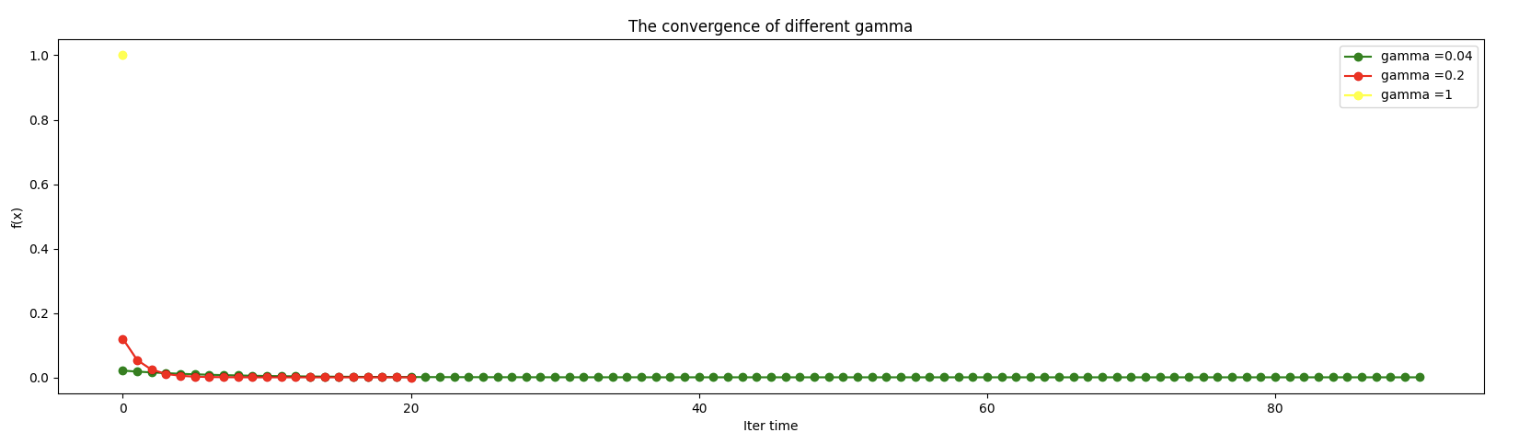
\includegraphics[width=0.7\textwidth]{quar1.png}
    \caption*{Value of f(x) and iteration time}
\end{figure}
从上图中看出当$\gamma = 1$时,一次迭代就得到最优解(黄色的点),当$\gamma$离1不远时(绿色曲线),收敛速度也很快,当$\gamma <<1 $,收敛速度相对较慢\\
\begin{figure}[H] 
    \centering 
    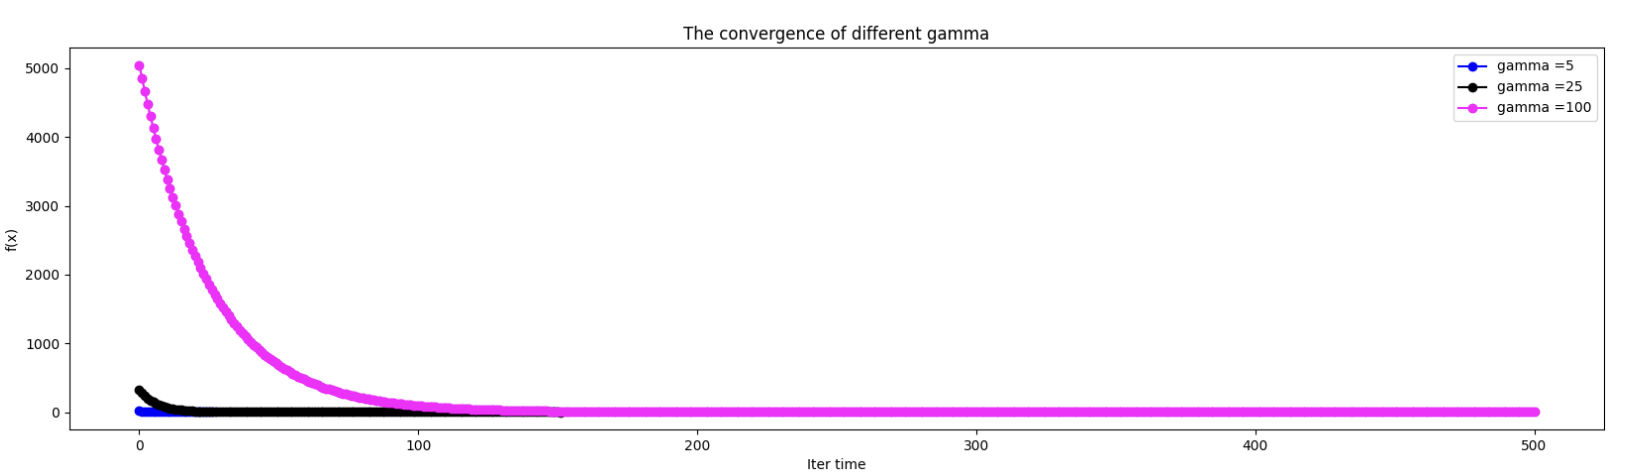
\includegraphics[width=0.7\textwidth]{quar2.png}
    \caption*{Value of f(x) and iteration time}
\end{figure}
当$\gamma >> 1$,收敛速度也很快非常慢(粉色曲线)
设定最小值误差$\epsilon = 1e-8$,不同$\gamma$值$f(x)$收敛次数为:
\begin{figure}[H] 
    \centering 
    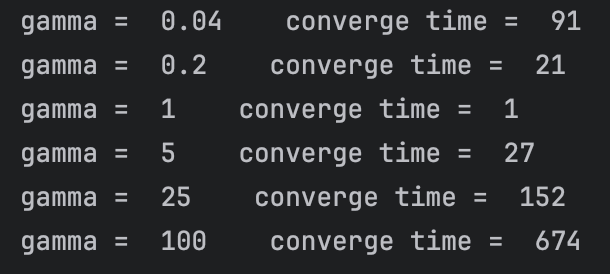
\includegraphics[width=0.7\textwidth]{quar3.png}
    \caption*{Convergence time}
\end{figure}


\newpage
{\centering\section*{大作业}}
对于$\mathbb{R}^2$空间非二次线性规划问题$min f(x) = e^{x_1 + 3x_2 -0.1} + e^{x_1 - 3x_2- 0.1 } + e^{-x_1-0.1}$,使用梯度下降法求解,分析:\\
(1)精确直线搜索时,目标函数值随迭代次数改变的情况\\
(2)回溯直线搜索时,设置不同的$\alpha,\beta$值,目标函数值随迭代次数改变的情况\\
解:
(1)设置初始值为$x_1 = 0.5, x_2 = 0.5$,使用精确直线搜索时,目标函数值随迭代次数变化的图像如图:\\
\begin{figure}[H] 
    \centering 
    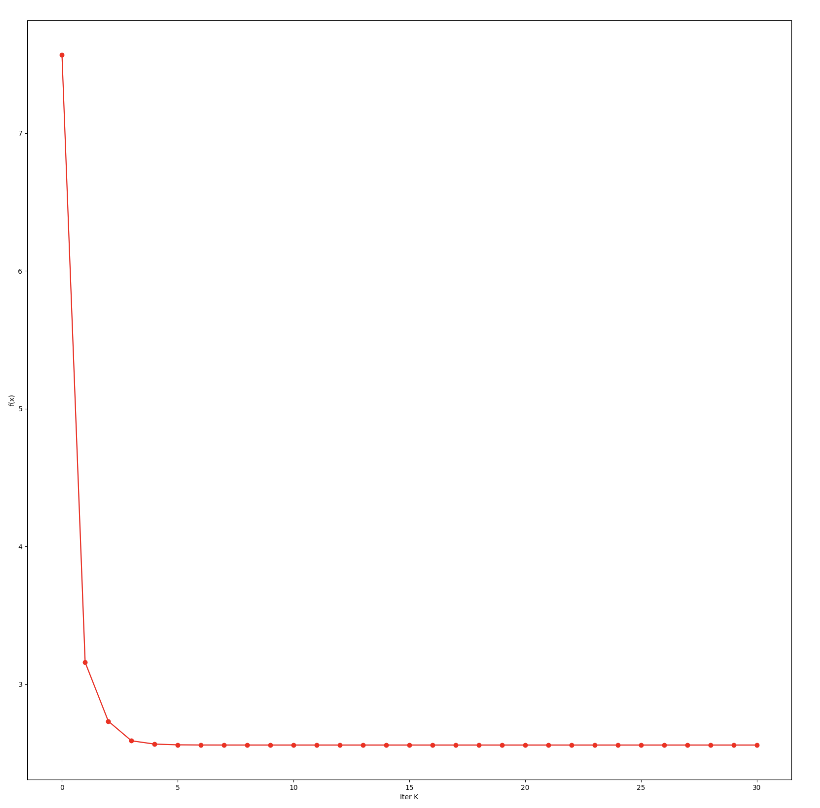
\includegraphics[width=0.8\textwidth]{ELS.png}
    \caption*{ExactLinearSearch}
\end{figure}
我们可以看到,$f(x)$的值在精确直线搜索前期快速收敛至最优值附近,之后缓慢变化,在10次左右便与最优值相差非常小。

(2)设置初始值为$x_1 = 0.5, x_2 = 0.5$,使用回溯直线搜索时,目标函数值随迭代次数变化的图像如图(设置$\epsilon = 1e-10$,观察不同$\alpha,\beta$下函数$f(x)$收敛次数):\\
\begin{figure}[H] 
    \centering 
    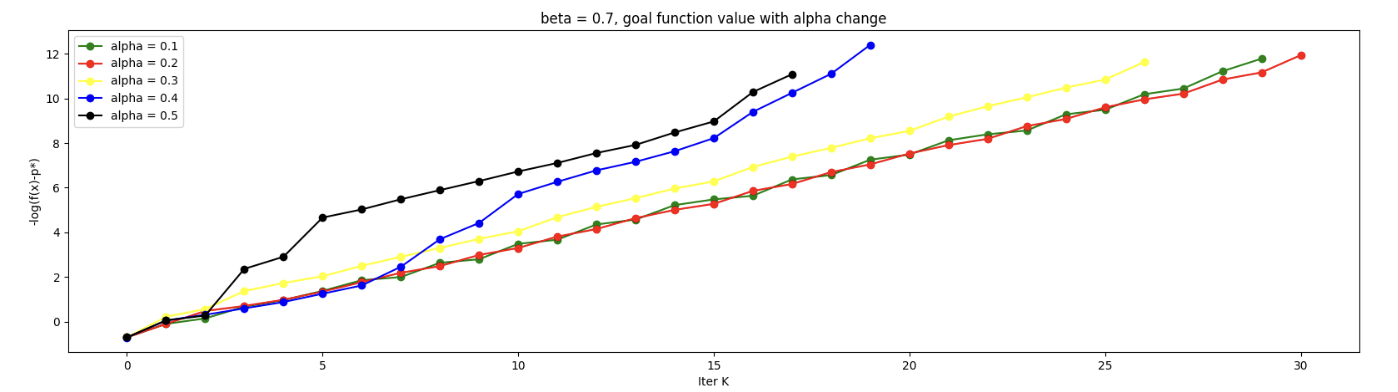
\includegraphics[width=0.8\textwidth]{Backtracking1.png}
    \caption*{Backtracking}
\end{figure}
从上图中可以看出当$\beta = 0.7$时,收敛次数随着$\alpha$的值的增大而减小。因为$\alpha$的值越大,意味着对下降的要求越严格,故收敛次数越少。

\begin{figure}[H] 
    \centering 
    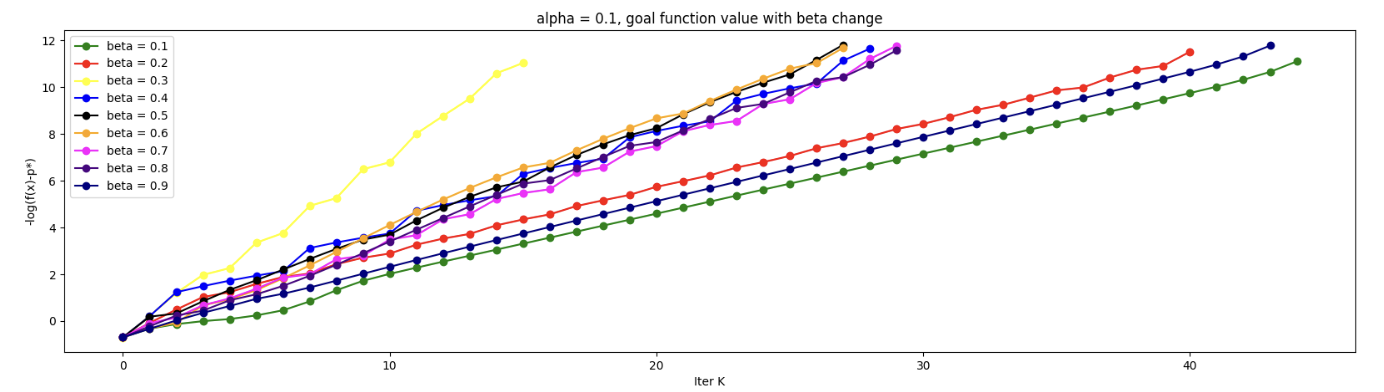
\includegraphics[width=0.8\textwidth]{Backtracking2.png}
    \caption*{Backtracking}
\end{figure}
从上图中可以看出当$\alpha = 0.1$时,收敛次数在$\beta = 0.3 $时最小。在$\beta < 0.3 $时,随$\beta$的增大而减小;在$\beta >0.3 $时,随$\beta$的增大而增大\\

精确直线搜索和回溯直线搜索不同参数的最终函数最优值与迭代次数如下图:
\begin{figure}[H] 
    \centering 
    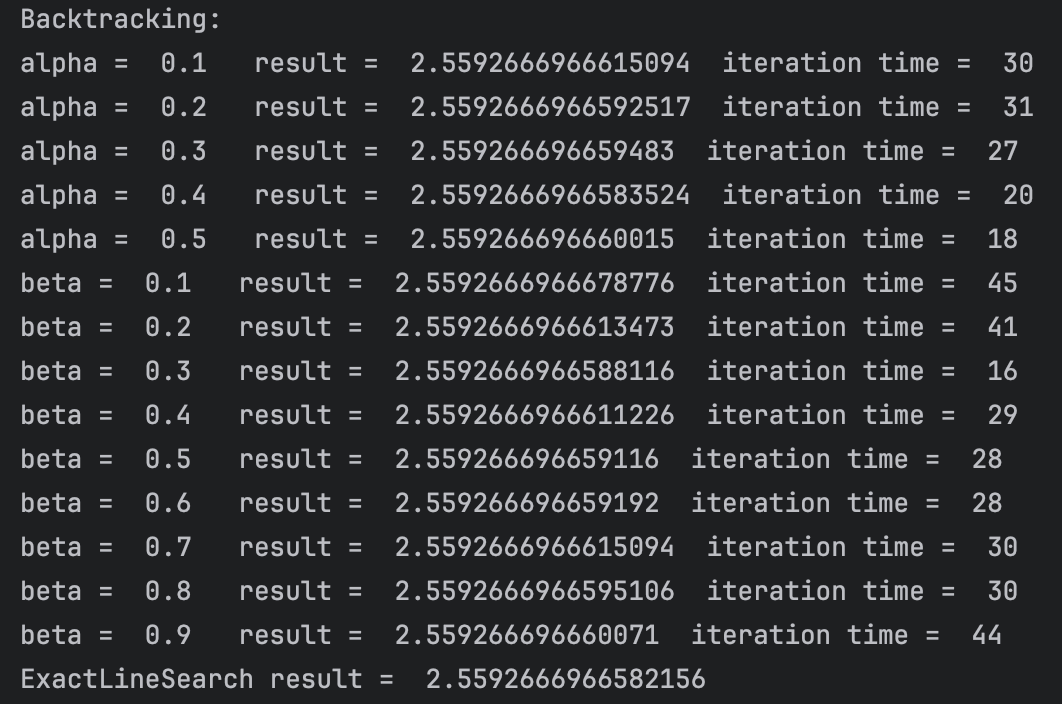
\includegraphics[width=0.8\textwidth]{res.png}
    \caption*{Result}
\end{figure}
可以看到,无论是精确直线搜索还是回溯直线搜索,都可以找到优化问题的最优解。且不同参数找到最优解的迭代次数不同。

\newpage
\lstdefinestyle{Python}{
    language        =   Python,
    basicstyle      =   \zihao{-5}\ttfamily,
    numberstyle     =   \zihao{-5}\ttfamily,
    keywordstyle    =   \color{blue},
    keywordstyle    =   [2] \color{teal},
    stringstyle     =   \color{magenta},
    commentstyle    =   \color{red}\ttfamily,
    breaklines      =   true,  
    columns         =   fixed,  
    basewidth       =   0.5em,
}

{\section*{附录}}
1.二次规划问题代码
\begin{lstlisting}

    import numpy as np
    import matplotlib.pyplot as plt
    # 定义目标函数及其梯度
    def f(x, gamma):
        return 0.5 * (x[0]**2 + gamma * x[1]**2)
    def grad_f(x, gamma):
        res = [x[0],gamma * x[1]]
        return res
    def gradient_descent(Max_iter,gamma):
        y_plot = []
        epsilon = 1e-8
        x = [gamma,1]
        y = f(x,gamma)
        y_plot.append(y)
        t = 2 / (1 + gamma)
        iteration_count = 0
        converge_time = Max_iter
        while(iteration_count < Max_iter):
            gradient = grad_f(x,gamma)
            for i in range(len(gradient)):
                gradient[i] = gradient[i] * t

            for i in range(len(gradient)):
                x[i] = x[i] - gradient[i]
            y = f(x,gamma)
            iteration_count += 1
            if(y < epsilon):
                converge_time = iteration_count
                break
            y_plot.append(y)
        return y_plot, converge_time
    if __name__ == '__main__':
        plt.figure(1,figsize=(20, 5))
        gamma_list = [0.04,0.2,1]
        max_iter = 5000
        color = ['green', 'red', 'yellow']
        legend = []
        for i in range(len(gamma_list)):
            y,converge_time = gradient_descent(max_iter,gamma_list[i])
            print('gamma = ',gamma_list[i],end='    ')
            print('converge time = ',converge_time)
            legend.append('gamma =' + str(gamma_list[i]))
            plt.plot(y, color = color[i], marker = 'o',linestyle = '-')
        plt.xlabel("Iter time")
        plt.ylabel("f(x)")
        plt.legend(legend)
        plt.title("The convergence of different gamma")
        plt.show()
        plt.figure(2, figsize=(20, 5))
        gamma_list = [5,25,100]
        color = ['blue', 'black', 'fuchsia']
        legend = []
        for i in range(len(gamma_list)):
            y,converge_time = gradient_descent(max_iter, gamma_list[i])
            print('gamma = ',gamma_list[i],end='    ')
            print('converge time = ',converge_time)
            legend.append('gamma =' + str(gamma_list[i]))
            plt.plot(y, color=color[i], marker='o', linestyle='-')
        plt.xlabel("Iter time")
        plt.ylabel("f(x)")
        plt.legend(legend)
        plt.title("The convergence of different gamma")
        plt.show()

    \end{lstlisting}

\newpage
2. 大作业代码:

\begin{lstlisting}
    import matplotlib.pyplot as plt
    from math import exp, log10
    import numpy as np
    from scipy.optimize import minimize_scalar
    
    
    def Func(x1, x2):
        res = exp(x1 + 3 * x2 - 0.1) + exp(x1 - 3 * x2 - 0.1) + exp(-x1 - 0.1)
        return res
    
    
    def grad_func(x1, x2):
        res = [exp(x1 + 3 * x2 - 0.1) + exp(x1 - 3 * x2 - 0.1) - exp(-x1 - 0.1),
               3 * exp(x1 + 3 * x2 - 0.1) - 3 * exp(x1 - 3 * x2 - 0.1)]
        return res
    
    
    def backtracking(alpha, beta):  # 回溯直线搜索
        x1 = x2 = 0.5
        y = Func(x1, x2)
        maxIter = 300
    
        curve2 = [y]
        iterationcount = 0
        gradient = grad_func(x1, x2)
        epsilon = 1e-5
        while (gradient[0] ** 2 + gradient[1] ** 2 > epsilon * epsilon and iterationcount < maxIter):
            iterationcount += 1
            gradient = grad_func(x1, x2)
            # 找t_k
            t_k = 1.0
            while (Func(x1 - t_k * gradient[0], x2 - t_k * gradient[1]) >
                   y - alpha * t_k * (gradient[0] ** 2 + gradient[1] ** 2)):
                t_k *= beta
            x1 = x1 - t_k * gradient[0]
            x2 = x2 - t_k * gradient[1]
            y_iter = Func(x1, x2)
            y = y_iter
    
            curve2.append(y)
        y_star = y
        # calculate distance between points form curve2 to y*
        for i in range(len(curve2)):
            curve2[i] -= y_star
        return curve2, y_star, iterationcount
    
    
    def backtracking_show():  # 回溯直线搜索绘图
        print("Backtracking:")
        # alpha change
        plt.figure(1, figsize=(20, 5))
        index = 0
        color = ['green', 'red', 'yellow', 'blue', 'black', 'orange', 'fuchsia', 'indigo', 'navy', 'gray']
        legend = []
        while (index <= 4):
            alpha = (index + 1) / 10
            curve, y, k = backtracking(alpha, 0.7)
            for i in range(len(curve) - 1):
                curve[i] = -1 * log10(curve[i])
            curve.pop()
            plt.plot(curve, color=color[index], marker='o')
            print("alpha = ", alpha, end='   ')
            print("result = ", y, end='  ')
            print("iteration time = ", k)
            legend.append("alpha = " + str(alpha))
            index += 1
        plt.xlabel("Iter K")
        plt.ylabel("-log(f(x)-p*)")
        plt.legend(legend)
        plt.title("beta = 0.7, goal function value with alpha change")
        plt.show()
    
        # beta change
        plt.figure(2, figsize=(20, 5))
        index = 0
        legend = []
        color = ['green', 'red', 'yellow', 'blue', 'black', 'orange', 'fuchsia', 'indigo', 'navy', 'gray']
        while (index <= 8):
            beta = (index + 1) / 10
            curve, y, k = backtracking(0.1, beta)
            for i in range(len(curve) - 1):
                curve[i] = -1 * log10(curve[i])
            curve.pop()
            plt.plot(curve, color=color[index], marker='o')
            print("beta = ", beta, end='   ')
            print("result = ", y, end='  ')
            print("iteration time = ", k)
            legend.append("beta = " + str(beta))
            index += 1
        plt.xlabel("Iter K")
        plt.ylabel("-log(f(x)-p*)")
        plt.legend(legend)
        plt.title("alpha = 0.1, goal function value with beta change")
        plt.show()
        return
    
    
    def ExactLineSearch():  # 精确直线搜索
        x1 = x2 = 0.5
        y = Func(x1, x2)
        maxIter = 30
    
        curve = [y]
        iterationcount = 0
        while (iterationcount < maxIter):
            iterationcount += 1
            gradient = grad_func(x1, x2)
    
            def line_search(alpha):
                return Func(x1 - alpha * gradient[0], x2 - alpha * gradient[1])
    
            res = minimize_scalar(line_search)
            alpha_opt = res.x  # optimal t
    
            x1 = x1 - alpha_opt * gradient[0]
            x2 = x2 - alpha_opt * gradient[1]
    
            cur_res = Func(x1, x2)
            curve.append(cur_res)
        return curve, cur_res
    
    
    def ExactLineSearch_show():
        plt.figure(figsize=(20, 20))
        curve, y = ExactLineSearch()
        plt.plot(curve, color='red', marker='o')
        print("ExactLineSearch result = ", y, end='  ')
        plt.xlabel("Iter K")
        plt.ylabel("f(x)")
        # plt.title("f(x) with change of iterate times")
        plt.show()
    
    
    backtracking_show()
    ExactLineSearch_show()
    
    \end{lstlisting}

\end{document}
